\documentclass[11pt,a4paper]{article}

\usepackage[utf8]{inputenc}
\usepackage[T1]{fontenc}
\usepackage{lmodern}
\usepackage[french]{babel}
\usepackage[margin=2.3cm]{geometry}
\usepackage{graphicx}
\usepackage{booktabs}
\usepackage{listings}
\usepackage{xcolor}
\usepackage{hyperref}
\usepackage{microtype}

\hypersetup{colorlinks=true,linkcolor=black,urlcolor=blue,plainpages=false}

\lstset{
  basicstyle=\ttfamily\small,
  frame=single,
  framerule=0.4pt,
  rulecolor=\color{black!30},
  backgroundcolor=\color{black!3},
  columns=fullflexible,
  keepspaces=true,
  aboveskip=6pt,
  belowskip=4pt
}

% Les pages ne contenant qu'un flottant : alignement en haut de page
\makeatletter
\setlength{\@fptop}{0pt}
\setlength{\@fpsep}{8pt plus 1fil}
\setlength{\@fpbot}{0pt plus 1fil}
\makeatother

\setlength{\parskip}{3pt}
\setlength{\parindent}{0pt}

\begin{document}

% Page de garde : non comptée dans les pages du rapport (la numérotation
% redémarre à 1 après l'environnement titlepage).
\begin{titlepage}
\centering
\vspace*{1cm}


\includegraphics[width=5.5cm]{insat_logo.jpg}

\vspace{0.8cm}
{\large Institut National des Sciences Appliquées et de Technologie}

\vspace{1.2cm}
\rule{\textwidth}{0.6pt}

\vspace{0.6cm}
{\Large Mini-projet 1}

\vspace{0.5cm}
{\Huge\bfseries Accélérateur IA minimal}

\vspace{0.4cm}
{\LARGE MAC + ReLU en HDL (Verilog)}

\vspace{0.6cm}
\rule{\textwidth}{0.6pt}

\vspace{1.5cm}
{\large Rapport de projet}

\vspace{1.5cm}
{\large Réalisé par :}

\vspace{0.3cm}
{\Large\bfseries Aziz Hizem}

\vspace{0.2cm}
{\Large\bfseries Manar Afli}

\vfill
{\large Année universitaire 2026--2027}

\vspace{0.3cm}
{\large \today}
\end{titlepage}

\section{Objectif}

Les réseaux de neurones reposent sur une opération élémentaire : la somme pondérée
$\sum_i a_i \times b_i$, suivie d'une fonction d'activation. Ce projet conçoit en
Verilog un accélérateur matériel minimal pour ces deux opérations :
une unité \emph{MAC} (Multiply-Accumulate) et une activation \emph{ReLU},
$\mathrm{ReLU}(x)=\max(0,x)$. Le circuit est vérifié par un testbench HDL, par un
modèle Python de référence et par des tests automatisés cocotb.

Le code, les tests et ce rapport sont disponibles sur GitHub :

\begin{center}
\small\url{https://github.com/aziz-hizem/soc-mac-relu-accelerator}
\end{center}

\section{Outils}

\begin{center}
\begin{tabular}{@{}ll@{}}
\toprule
Outil & Rôle \\
\midrule
Icarus Verilog 12 & compilation et simulation du Verilog \\
GTKWave & visualisation des chronogrammes (fichiers VCD) \\
Verilator 5 & analyse statique (\emph{lint}) du code HDL \\
Python, NumPy & modèle de référence \\
cocotb 2.1.0 & tests automatisés du circuit en Python \\
\bottomrule
\end{tabular}
\end{center}

\section{Conception}

Le module \texttt{mac\_relu} (fichier \texttt{mac\_relu.v}) possède une horloge
\texttt{clk}, un reset asynchrone \texttt{reset}, deux entrées signées sur 8 bits
\texttt{a} et \texttt{b}, un accumulateur signé sur 32 bits \texttt{acc} et la
sortie \texttt{relu\_out}. À chaque front montant de l'horloge :
\[
\texttt{acc} \leftarrow \texttt{acc} + a \times b, \qquad
\texttt{relu\_out} = \max(0,\texttt{acc}).
\]

Le produit $a\times b$ est calculé sur 16 bits signés, puis étendu en signe sur
32 bits avant l'addition ; sans cette extension, les produits négatifs seraient
mal accumulés. La sortie ReLU est combinatoire.

\begin{lstlisting}[language=Verilog,morekeywords={always,posedge,assign,wire,signed}]
wire signed [15:0] produit = a * b;

always @(posedge clk or posedge reset) begin
    if (reset) acc <= 32'sd0;
    else       acc <= acc + {{16{produit[15]}}, produit};
end

assign relu_out = (acc > 0) ? acc : 32'sd0;
\end{lstlisting}

\section{Vérification}

La vérification repose sur trois niveaux complémentaires, qui utilisent les mêmes
vecteurs de test (huit couples $(a,b)$, dont les cas limites
$(-128)\times(-128)$ et $127\times127$).

\begin{itemize}
  \item \textbf{Testbench Verilog} (\texttt{tb\_mac\_relu.v}) : il est
  auto-vérifiant. Il applique les huit vecteurs, compare \texttt{acc} et
  \texttt{relu\_out} aux valeurs attendues, teste le reset puis affiche
  \texttt{TOUS LES TESTS ONT REUSSI} ou le nombre d'erreurs. Il écrit aussi le
  fichier VCD utilisé pour le chronogramme.
  \item \textbf{Modèle Python} (\texttt{vectors.py}, \texttt{reference.py}) :
  le modèle calcule le produit, l'accumulation et la ReLU cycle par cycle ;
  \texttt{reference.py} affiche le tableau de référence avec NumPy.
  \item \textbf{Tests cocotb} (\texttt{test\_mac\_relu.py}) : un premier test
  rejoue les huit vecteurs ; un second applique 500 cycles aléatoires (graine
  fixe 2026) avec un reset au cycle 250. À chaque cycle, \texttt{acc} et
  \texttt{relu\_out} sont comparés au modèle Python.
\end{itemize}

Pour contrôler que le testbench détecte bien les erreurs, nous avons introduit
volontairement un défaut (suppression de l'extension de signe) dans une copie du
module : le testbench signale alors une erreur sur chacun des huit cycles.

\section{Résultats}

Le tableau~\ref{tab:res} donne les valeurs obtenues. Elles sont identiques dans le
testbench Verilog, dans le modèle Python et dans les tests cocotb. Les deux
premières sommes sont négatives et la ReLU les ramène à zéro.

\begin{table}[h]
\centering
\caption{Résultats de simulation (identiques pour Verilog, Python et cocotb).}
\label{tab:res}
\begin{tabular}{@{}rrrrrr@{}}
\toprule
Cycle & $a$ & $b$ & Produit & ACC & ReLU \\
\midrule
1 & $-3$   & 4    & $-12$   & $-12$ & 0 \\
2 & 2      & 3    & 6       & $-6$  & 0 \\
3 & 5      & 4    & 20      & 14    & 14 \\
4 & $-2$   & 3    & $-6$    & 8     & 8 \\
5 & $-128$ & $-128$ & 16384 & 16392 & 16392 \\
6 & 127    & 127  & 16129   & 32521 & 32521 \\
7 & 0      & 5    & 0       & 32521 & 32521 \\
8 & $-128$ & 1    & $-128$  & 32393 & 32393 \\
\bottomrule
\end{tabular}
\end{table}

\begin{figure}[t]
\centering
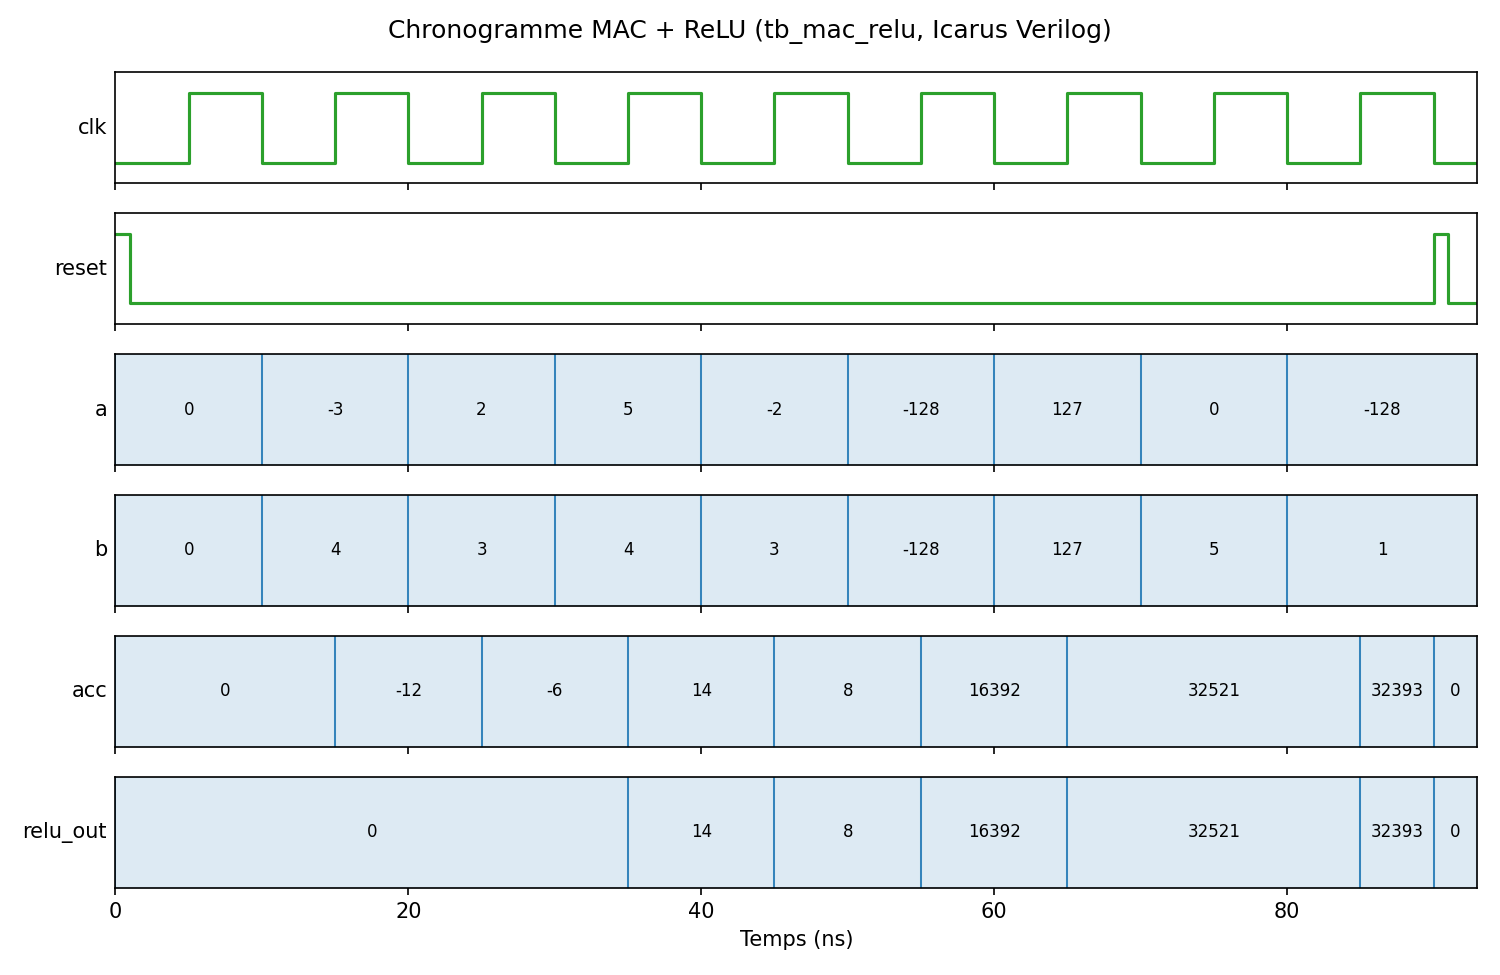
\includegraphics[width=\textwidth]{../docs/chronogramme.png}
\caption{Chronogramme de la simulation : horloge, reset, entrées $a$ et $b$,
accumulateur et sortie ReLU (valeurs en décimal signé).}
\label{fig:chrono}
\end{figure}

La figure~\ref{fig:chrono} montre que l'accumulateur se met à jour à chaque front
montant de l'horloge et que \texttt{relu\_out} reste à zéro tant que \texttt{acc}
est négatif. Les chronogrammes ont été observés avec GTKWave pendant le
développement ; la figure finale est tracée par un script Python
(\texttt{plot\_waveform.py}) à partir du fichier VCD, ce qui la rend reproductible.

Le cocotb signale \texttt{TESTS=2 PASS=2 FAIL=0}. L'analyse Verilator
(\texttt{--lint-only -Wall}) du module et du testbench ne produit aucun
avertissement.

\section{Limites et conclusion}

L'accumulateur est signé sur 32 bits et ne détecte pas le débordement : avec des
entrées sur 8 bits, il pourrait déborder après environ $2^{31}/2^{14}=131\,072$
produits maximaux consécutifs. Le reset est asynchrone, ce qui convient à ce
circuit simple. Les entrées sont des entiers sur 8 bits ; un vrai accélérateur
manipulerait des vecteurs et plusieurs unités MAC en parallèle.

Le projet répond au cahier des charges : une unité MAC avec ReLU, un testbench
HDL auto-vérifiant, un modèle Python de référence avec comparaison automatique
(cocotb), des chronogrammes et une analyse statique Verilator. Toutes les
vérifications réussissent sur les cas testés.

\end{document}
